\section{Sensoriamento} % (fold)
\label{sec:sensoriamento2}

	Após definir as especificações dos componentes na sessão \ref{sec:sensoriamento}, será descrito a seguir de forma detalhada as estratégias seguidas pelo grupo para atender aos requisitos do projeto. Tambem serão apresentadas as simulações realizadas para validar os conceitos aplicados, resultados práticos serão apresentados em um momento posterior.

	A parte do projeto de eletrônica responsável pela comunicação será apresentada na sessão \ref{sub:hardware}.

	\subsection{Instrumentação} % (fold)
	\label{sub:instrumentação2}
		A instrumentação foi dividida em três subgrupos, cada um com um foco especifico para garantir a integridade do robô R2-PI2, esses subgrupos são apresentados a seguir.

		\subsubsection{Controle de distância}
		\label{sub:Controle_de_distância}
		A estratégia de controle utilizada na locomoção do R2-PI2, analisa as seguintes situações, o robô se locomoverá sempre para a frente enquanto não encontrar obstáculos em seu caminho. Na detecção de um objeto, os sensores posicionados a direta e a esquerda do robô farão a medição de distância. O aspirador tomará a decisão de desviar para o lado contrário da menor distância medida ou na ausência da mesma. Na possibilidade de ausência de distância ou impossibilidade de cálculos, o desvio será feito a direita por padrão. A figura \ref{img:fluxograma_eletronica} mostra o fluxograma do algoritmo utilizado na locomoção do aspirador.

		\begin{figure}[H]
			\centering
			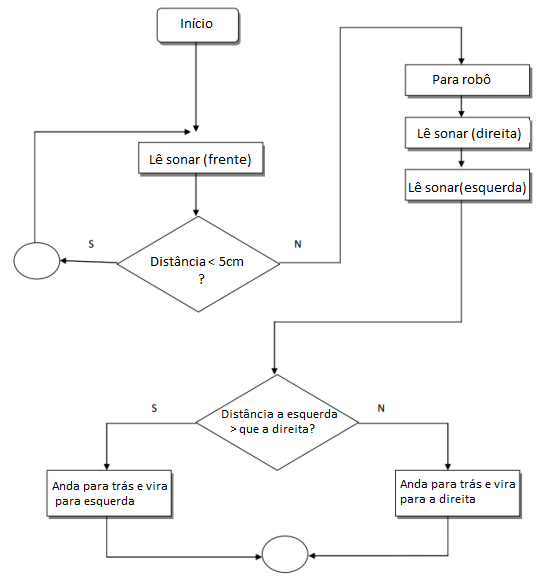
\includegraphics[scale=0.8]{figuras/fluxograma_eletronica.png}
			\caption{Fluxograma do algoritmo de locomoção do R2-PI2, realizado pela equipe de eletrônica para testes iniciais.}
			\label{img:fluxograma_eletronica}
		\end{figure}

		No caso da identificação de degraus ou desníveis o algoritmo consiste na simples análise de obstáculos ou não. Por limitação do sensor IR, a distância máxima medida é de 2.5 cm, então enquanto uma distância escolhida como aproximadamente 1cm estiver sendo medida, o que significa que o robô está em contato com o chão, ele continuará se movimentando normalmente, quando essa distância medida for maior que 1 cm, o aspirador irá parar, dar uma ré e escolher a melhor rota para continuar seguindo.

		Tanto no código de medição de distância com o ultrassom, quanto no com sensor IR utilizou-se a técnica de filtragem por médias móveis que consiste em fazer várias amostragens de um parâmetro e depois tirar a média das mesmas. O filtro ajudou bastante no problema de leituras oscilantes nos sensores. 

		\subsubsection{Monitoramento da bateria}
		\label{sub:Monitoramento_da_bateria}
		Com carga máxima, a bateria escolhida terá 12,6V e ela deixará de fornecer a corrente adequada ao circuito quando chegar a 8,25V (aproximadamente 66\% da bateria total). Para evitar que a bateria chegue a 8,25V no meio da execução da limpeza, um circuito comparador de tensão irá verificar continuamente qual a voltagem da bateria.

		Além de enviar o sinal para o microcontrolador, será feita uma interface visual com 5 LEDs que vão indicar quando a bateria está com carga total e quando a bateria está perto da carga mínima (8,25V), conforme a figura \ref{img:faixa_de_tensão}.

		\begin{figure}[H]
			\centering
			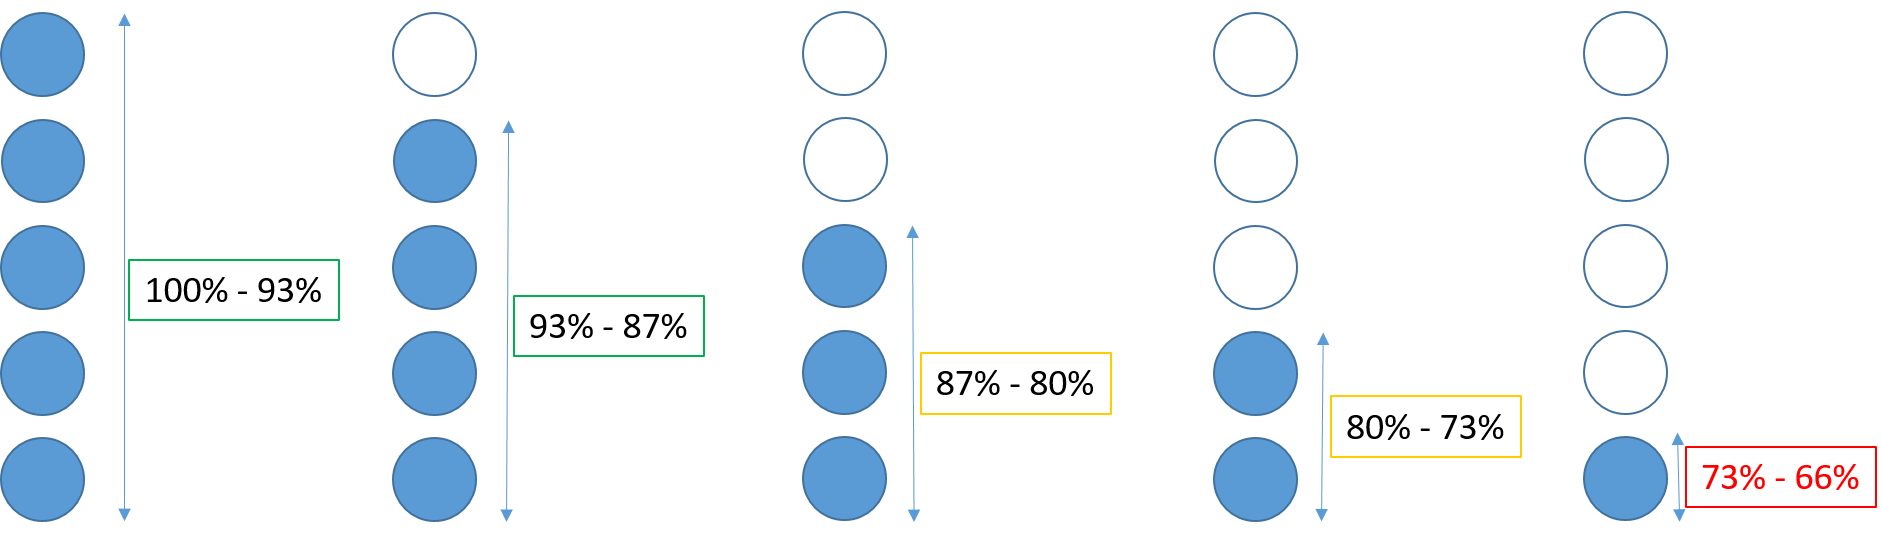
\includegraphics[scale=0.3]{figuras/LEDs.png}
			\caption{Aproximação das faixas de tensão apresentadas pelos LEDs.}
			\label{img:faixa_de_tensão}
		\end{figure}

		A queda de tensão será apresentada em cinco LEDs que foram divididos em faixas muito próximas de tensão útil. Conforme os seguintes cálculos:

		\begin{equation}
		\label{eq:equação_medidor_bateria}
			\frac{Tensão\ máxima - tensão\ mínima}{5}  
		\end{equation}

		Substituindo os valores em (\ref{eq:equação_medidor_bateria}), temos:

		\begin{equation}
		\label{eq:equação_medidor_bateria_2}
			\frac{100-66}{5} = 6,8  
		\end{equation}

		As faixas então foram definidas como:

		\begin{itemize}
			\item \textbf{Faixa 1}: 100\% $\sim$ 93,2\%
			\item \textbf{Faixa 2}: 93,2\% $\sim$ 86,4\%
			\item \textbf{Faixa 3}: 86,4\% $\sim$ 79,6\%
			\item \textbf{Faixa 4}: 79,6\% $\sim$ 72,8\%
			\item \textbf{Faixa 5}: 72,8\% $\sim$ 66\%
		\end{itemize}
		
		Considerando que o sistema de sucção consome cerca de seis vezes mais corrente do que o sistema de navegação do robô e que são cinco faixas de tensão, estimou-se que um quinto da tensão útil é suficiente para o robô voltar para a base de carregamento com o sistema de sucção desligado. No entanto, sabendo que a curva de descarga de uma bateria não é linear, apenas após os testes empíricos será possível determinar com maior segurança se um ou dois quintos da tensão útil serão colocados à disposição do sistema de navegação para o robô poder retornar à base. 

		Assim, enquanto a tensão da bateria estiver dentro das quatro faixas de tensão, o robô estará executando a rotina de limpeza e quando estiver na última faixa ele estará retornando para a base. 

		As faixas de tensão foram projetadas a partir de um divisor de tensão com cinco saídas sendo que cada saída é o limite inferior da faixa.

		\begin{figure}[H]
			\centering
			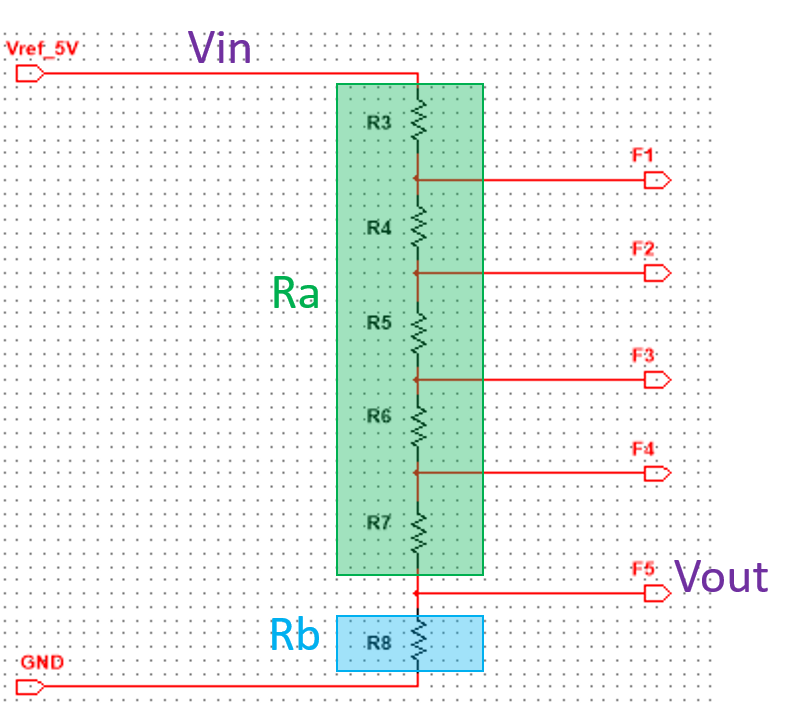
\includegraphics[scale=0.5]{figuras/Divisor1.png}
			\caption{Divisor de tensão.}
			\label{img:divisor_de_tensão}
		\end{figure}

		Fazendo o divisor de tensão com Ra e Rb, tem-se que:

		\begin{equation}
		\label{eq:divisor_de_tensão}
			Vout= \frac{Rb * Vin}{Ra + Rb} 
		\end{equation}

		Sabendo que ${Vout = 0,66 * Vin}$, substituimos \textit{Vout} na equação \ref{eq:divisor_de_tensão}:
		
		\begin{equation}
		\label{eq:divisor_de_tensão_2}
			0,66 *Vin=\frac{Rb *Vin}{Ra + Rb} 
		\end{equation}

		Que resulta em:

		\begin{equation}
		\label{eq:divisor_de_tensão_3}
			0,66 * Ra + 0,66 * Rb = Rb
		\end{equation}

		Se Rb=10K$\Omega$, substituimos na equação \ref{eq:divisor_de_tensão_3} e obtemos:

		\begin{equation}
		\label{eq:divisor_de_tensão_4}
			Ra=\frac{10K - 0,66 * 10K}{0,66} \simeq 5K
		\end{equation}

		Como as faixas devem ter a aproximadamente a mesma variação de tensão, os resistores R3, R4, R5, R6 e R7 devem ter o mesmo valor e sua associação em série deve ser igual a 5K$\Omega$ (Ra), assim os valores das resistências do divisor de tensão devem ser:

		\begin{equation}
		\label{eq:divisor_de_tensão_5}
			R3 + R4 + R5 + R6 + R7 = 5K\ =>\  
			R3 = R4 = R5 = R6 = R7 = 1K
		\end{equation}

		\begin{equation}
		\label{eq:divisor_de_tensão_6}
			Rb = Rc = 10K
		\end{equation}

		Para confirmar se o divisor proposto realmente cumpre os requisitos do projeto, foi realizada a simulação utilizando o software MultiSim do divisor aplicando uma tensão de 10V e o resultado obtido foi satisfatório.

		\begin{figure}[H]
			\centering
			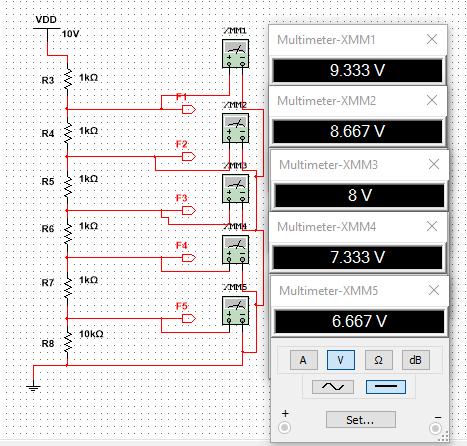
\includegraphics[scale=0.8]{figuras/Divisor1_simu.png}
			\caption{Simulação do divisor de tensão.}
			\label{img:divisor_de_tesnão_simulado}
		\end{figure}


		Para o circuito acima funcionar bem, a tensão de entrada do divisor de tensão deverá ser igual a tensão máxima da bateria. Como a tensão máxima da bateria é de 12.6V, fica inviável geral um sinal constante de 12.6V apenas para servir como referência do divisor. Sabendo que o ATMega gera um sinal de 5V, a tensão da bateria passará por um divisor de tensão  que será projetado para transformar os 12.6V em 5V de modo que seja possível utilizar os 5V do ATMega no medidor de bateria.

		Sabendo que a tensão de saída do novo resistor (Vout2) deve ser 5V e que a tensão de entrada (Vin2) é de 12.6V as resistências (Rc e Rd) utilizadas podem ser calculadas pela seguinte expressão:

		\begin{equation}
		\label{eq:divisor_de_tensão_7}
			Vout2 =\frac{Rc * Vin2}{Rc + Rd}
		\end{equation}

		Substituindo os valores em \ref{eq:divisor_de_tensão_7}, temos:

		\begin{equation}
		\label{eq:divisor_de_tensão_8}
			5\ =\frac{Rc * 12.6}{Rc + Rd}\ =>\ 7.6 * Rc = 5 *Rd
		\end{equation}

		Se Rc=1K$\Omega$, logo:

		\begin{equation}
		\label{eq:divisor_de_tensão_9}
			Rd =\frac{7.6}{5} \simeq 1.5K
		\end{equation}

		Para verificar o divisor projeto se adequa às necessidades do projeto, foi feita a simulação no software MultiSim e o resultado encontrado foi satisfatório. A variação de 0,04V corresponde a 0,3\% da tensão máxima e, portanto, não prejudicará o sistema de medição da bateria.

		\begin{figure}[H]
			\centering
			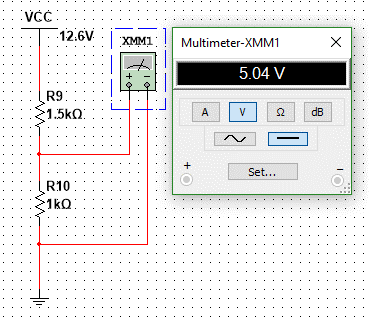
\includegraphics[scale=0.8]{figuras/Divisor2_simu.png}
			\caption{Simulação do divisor de tensão de 12.6V para 5V.}
			\label{img:divisor_de_tesnão_simulado}
		\end{figure}

		O circuito completo do medidor de bateria é apresentado na figura \ref{img:medidor_de_bateria}.

		\begin{figure}[H]
			\centering
			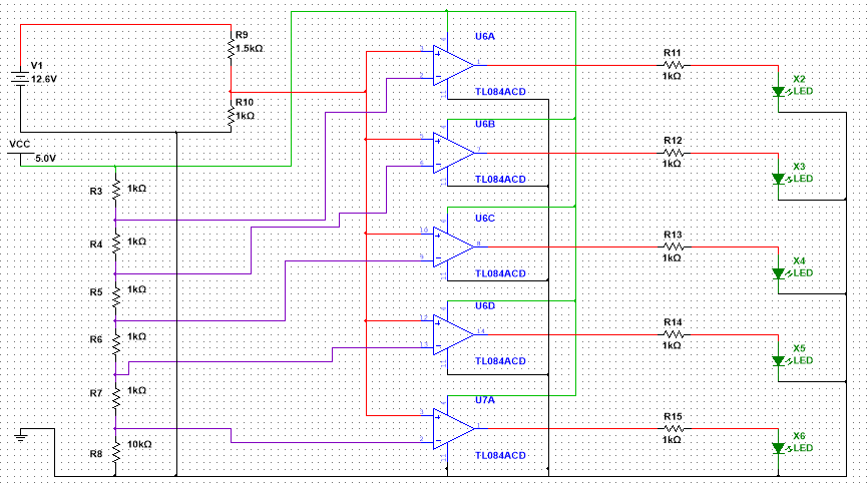
\includegraphics[scale=0.7]{figuras/Med_bateria.png}
			\caption{Circuito do medidor de bateria.}
			\label{img:medidor_de_bateria}
		\end{figure}

		\subsubsection{Proteção dos componentes}
		\label{sub:Proteção_dos_componentes_2}
		A porta lógica do ATMega envia até 40mA de corrente a 5V, para limitar a corrente que irá acionar o LED interno do acoplador óptico utilizaremos uma resistencia de 220$\Omega$. O outro lado do optoacoplador  terá uma resistor pull-up de 10K$\Omega$ para garantir que quando o fototransistor capte a luz, a corrente flua para o terra e ligue o motor do sistema de sucção.

		\begin{figure}[H]
			\centering
			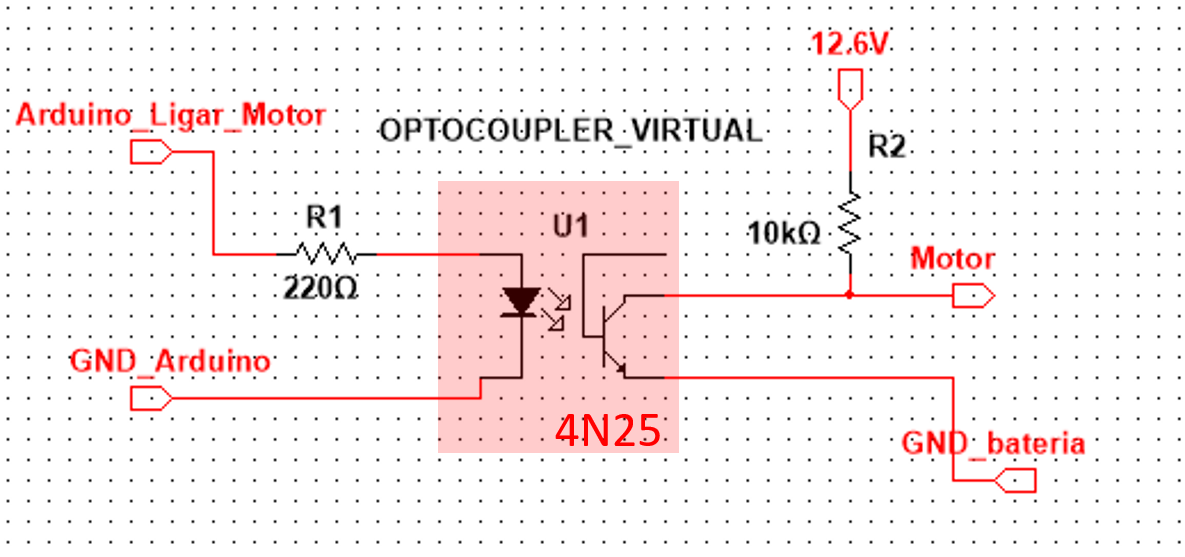
\includegraphics[scale=0.4]{figuras/simulacao_optacoplador.png}
			\caption{Circuito de proteção com acoplamento óptico.}
			\label{img:circuito_de_proteção}
		\end{figure}
	
	% subsection instrumentação (end)

	\subsection{Controle} % (fold)
	\label{sub:controle2}
		O sistema de controle descrito por meio do diagrama de blocos foi implementado utilizando-se os componentes e microcontrolador apresentados na proposta de solução. Abaixo encontra-se o esquemático detalhado do sistema de locomoção e desvio de obstáculos do aspirador. Como explicado anteriormente, foram utilizados quatro sensores ultrassônicos HC-SR04 que posicionam-se a 90º de distância um do outro. Os sensores possuem um ângulo de alcance de 15º e na forma como estão posicionados não cobrem todo o diâmetro do aspirador, no entanto, através de testes experimentais, percebeu-se que a quantidade e distribuição de sensores utilizados, assim como o algoritmo que foi implementado, atendem o requisito de desvio da maior parte dos obstáculos de um cômodo.

		Pode-se observar também no esquemático, o sensor TCRT5000 que foi posicionado na frente da roda boba afim de identificar algum degrau ou desnível que possa impedir o movimento do aspirador ou danificá-lo.

		\begin{figure}[H]
			\centering
			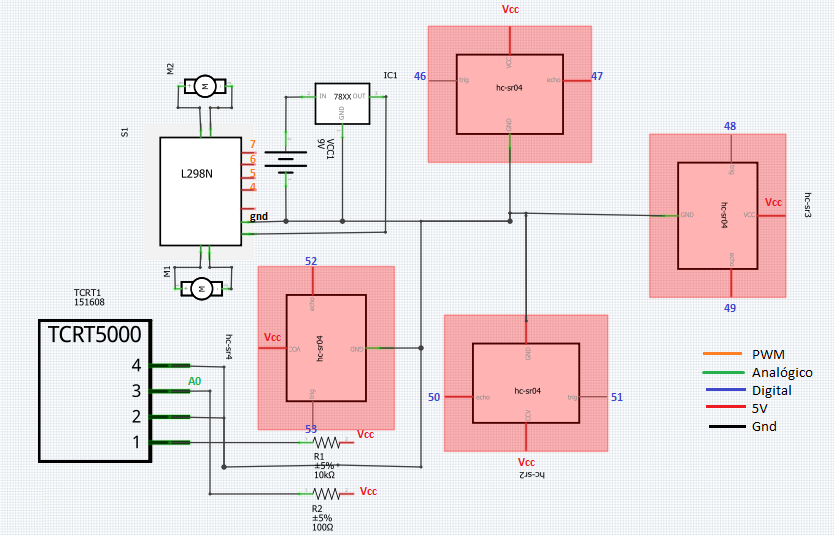
\includegraphics[scale=0.7]{figuras/locomocao1.png}
			\caption{Circuito de locomoção do aspirador.}
			\label{img:circuito_de_locmoção}
		\end{figure}

		Na montagem do circuito utilizou-se entradas analógicas, digitais e PWM. A legenda da figura identifica a natureza dos sinais utilizados de acordo com a pinagem do controlador.

		Os motores são controlados pela ponte H (L298N) que está conectada ao controlador por meio de entradas PWM. A ponte H permite a rotação dos motores nos dois sentidos e o controle de velocidade do mesmo. Sendo assim o aspirador pode se movimentar em todas as direções desviando-se de obstáculos e em uma velocidade adequada para que o sistema de sucção funcione de forma eficiente.

		Durante os testes de locomoção em conjunto com os sensores de obstáculos, observou-se que os sensores ultrassônicos e IR estavam variando muito , atrapalhando assim o movimento do aspirador. Após pesquisas concluiu-se que os motores estavam gerando ruído nos sensores e uma solução encontrada foi utilizar três capacitores cerâmicos de 100nF, um entre as escovas e os outros dois, cada um entre uma escova e a carcaça do motor. O esquema realizado para os dois motores se encontra na figura \ref{img:esquema_de_redução_de_ruido}.

		\begin{figure}[H]
			\centering
			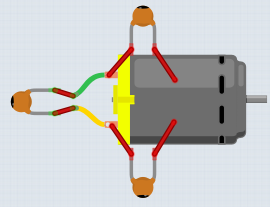
\includegraphics[scale=0.5]{figuras/motorcap.png}
			\caption{Esquema de redução de ruído do motor.}
			\label{img:esquema_de_redução_de_ruido}
		\end{figure}

		O controlador ATMega 2560 controla também o sistema de sucção do aspirador que conta com dois motores. Esse controle foi implementado por meio do chaveamento de transistores. O esquemático apresentado na figura \ref{img:circuito_de_controle_dos_motores} mostra o circuito de controle genérico dos motores do sistema.

		\begin{figure}[H]
			\centering
			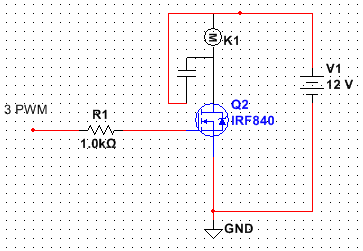
\includegraphics[scale=0.7]{figuras/chave.png}
			\caption{Circuito de controle dos motores.}
			\label{img:circuito_de_controle_dos_motores}
		\end{figure}

		O circuito é ativado por uma saída pwm do controlador que polariza o gate do transistor permitindo que ele conduza corrente através do motor. Por operar com uma corrente alta, utilizou-se um transistor de potência NMOS IRF840 que suporta uma corrente máxima de 8A e 500 V de tensão.

		O motor que ativa o sistema de sucção drena uma corrente muito alta, cerca de 4,4A. Caso haja uma corrente de fuga dos motores para o ATmega, o microcontrolador irá queimar instantaneamente, pois ele suporta até 500mA. Para garantir que essa situação não aconteça, será utilizado um circuito de proteção com optoacopladores, descrito na sessão \ref{sub:Proteção_dos_componentes_2}, que irá isola-lo eletricamente do motor.

	% subsection controle (end)
% section sensoriamento (end)

\subsection{Validação experimental} % (fold)
	\label{sub:validação_experimental}
	\begin{itemize}
		\item \textbf{Teste do controle sistema de controle + sistema de distância}

			Para testar o sistema de controle e validar seu funcionamento adequado, conectou-se os sensores ultrassônicos ao ATMega assim como a ponte H e os motores acoplados as rodas. Depois disso criou-se funções de locomoção com as direções básicas para os motores: frente, ré, esquerda, direita e parar. E criou-se um algoritmo para implementar o fluxograma feito no controle de distância. O algoritmo encontra-se disponível em \href{https://github.com/kaiocoelho/CodigoESP/blob/master/codigo_teste/Teste_ultrassom.ino}{Teste ultrassom}.

			Estando prontos os projetos de hardware e software, carregou-se o código no ATMega e ligou-se a fonte da ponte H. O carrinho então começou a andar e colocou-se obstáculos em sua frente observando que o controle e sensores estavam trabalhando de forma eficaz e desviando da maior parte dos obstáculos conforme o esperado.

		\item \textbf{Teste Medidor de Bateria}

			Com o circuito todo montado em uma \textit{protoboard}, sem o divisor de tensão inicial, inseriu-se uma tensão de 12V na entrada. Todos os cinco LEDs acenderam e conforme a tensão de entrada ia mudando de faixa de tensão, os LEDs respectivos iam apagando. O teste mostrou que o circuito funciona como o esperado.

			No entanto, esse circuito foi montado em uma placa impressa e ainda não foi testado com a bateria que será utilizada no protótipo.

			Para ajudar a faixa crítica de tensão, é necessário saber qual a tensão mínima real com todo o sistema do robô em funcionamento.

			Após integrar todo o sistema do robô, será necessário deixar todos os subsistemas funcionando até a bateria parar de fornecer a corrente necessária. Esse teste permitirá conhecer o seu tempo máximo de funcionamento e a tensão mínima para calibrar o medidor.

		\item \textbf{Teste do circuito de proteção}

			O circuito de proteção óptica foi testado colocando um arduino controlar um sistema alimentado a 9V.

			Nesse teste, foi possível perceber que o arduíno controla muito bem o circuito de 9V por meio do optoacoplador, mesmo sem o contato elétrico com os fios.

			O circuito ainda precisará ser testado com o sistema de sucção na fase de integração dos subsistemas. Nesse teste, será enviado um pulso do arduíno para acionar o motor do sistema de sucção.
	\end{itemize}

